\documentclass[tikz,border=4pt]{standalone}
\usepackage{amsmath,amssymb}
\usepackage{helvet}
\renewcommand{\familydefault}{\sfdefault}
\usetikzlibrary{positioning,arrows.meta,fit,backgrounds,calc,shapes.geometric}
\definecolor{cblue}{HTML}{0072B2}
\definecolor{corange}{HTML}{E69F00}
\definecolor{cgreen}{HTML}{009E73}
\definecolor{cred}{HTML}{D55E00}
\definecolor{cgrey}{HTML}{6E6E6E}
\definecolor{cpurple}{HTML}{CC79A7}
\begin{document}
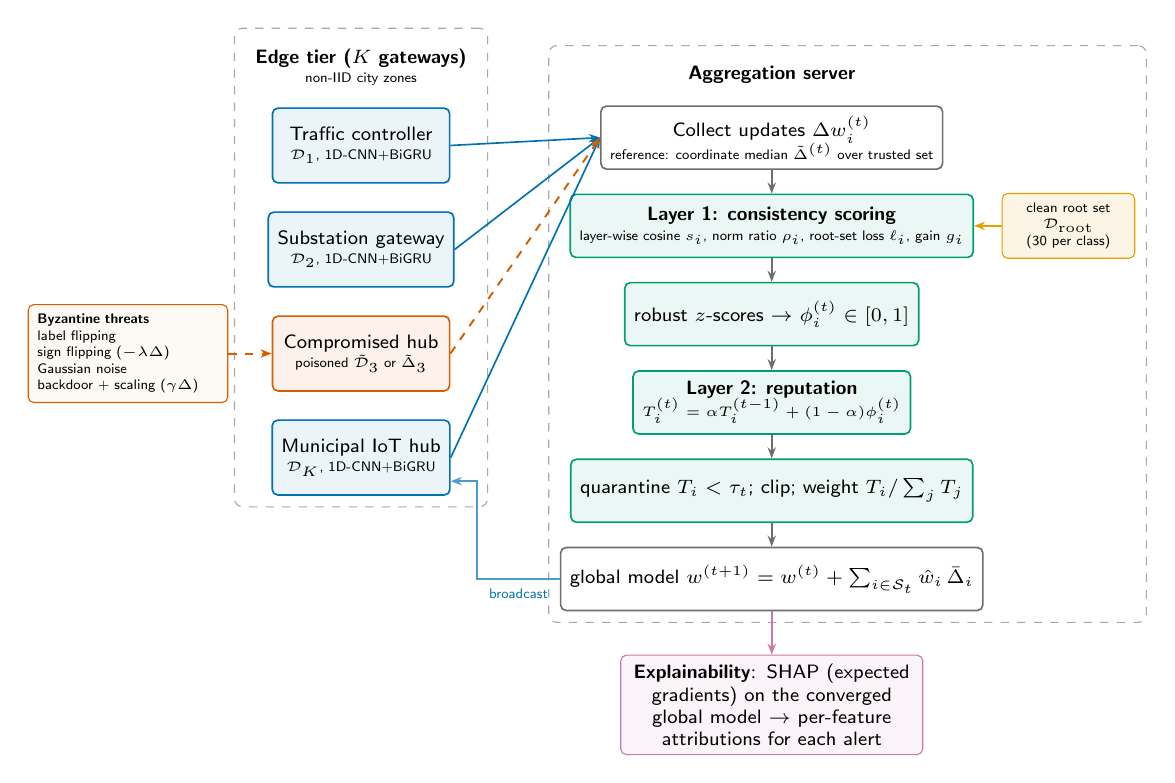
\begin{tikzpicture}[font=\scriptsize,
  gw/.style={draw=cblue,fill=cblue!8,rounded corners=2pt,minimum width=2.25cm,minimum height=0.95cm,align=center,line width=0.6pt},
  bad/.style={draw=cred,fill=cred!8,rounded corners=2pt,minimum width=2.25cm,minimum height=0.95cm,align=center,line width=0.6pt},
  blk/.style={draw=cgrey,fill=white,rounded corners=2pt,minimum width=3.3cm,minimum height=0.8cm,align=center,line width=0.6pt},
  hl/.style={draw=cgreen,fill=cgreen!8,rounded corners=2pt,minimum width=3.3cm,minimum height=0.8cm,align=center,line width=0.6pt},
  arr/.style={-{Stealth[length=4pt]},line width=0.6pt,color=cgrey},
  marr/.style={-{Stealth[length=4pt]},line width=0.7pt,color=cred,dashed}]

% ---------------- edge tier
\node[gw] (g1) {Traffic controller\\[-1pt]{\tiny $\mathcal{D}_1$, 1D-CNN+BiGRU}};
\node[gw,below=0.35cm of g1] (g2) {Substation gateway\\[-1pt]{\tiny $\mathcal{D}_2$, 1D-CNN+BiGRU}};
\node[bad,below=0.35cm of g2] (g3) {Compromised hub\\[-1pt]{\tiny poisoned $\tilde{\mathcal{D}}_3$ or $\tilde{\Delta}_3$}};
\node[gw,below=0.35cm of g3] (g4) {Municipal IoT hub\\[-1pt]{\tiny $\mathcal{D}_K$, 1D-CNN+BiGRU}};
\node[above=0.15cm of g1,font=\scriptsize\bfseries,align=center] (et) {Edge tier ($K$ gateways)\\[-1pt]{\tiny\mdseries non-IID city zones}};
\begin{scope}[on background layer]
\node[draw=cgrey!60,dashed,rounded corners=3pt,fit=(et)(g1)(g4),inner sep=4pt] (edge) {};
\end{scope}

% threat box
\node[draw=cred,fill=cred!4,rounded corners=2pt,align=left,left=0.55cm of g3,text width=2.3cm,font=\tiny] (thr) {\textbf{Byzantine threats}\\label flipping\\sign flipping ($-\lambda\Delta$)\\Gaussian noise\\backdoor + scaling ($\gamma\Delta$)};
\draw[marr] (thr.east) -- (g3.west);

% ---------------- server tier
\node[blk,right=1.9cm of g1,yshift=0.1cm] (rec) {Collect updates $\Delta w_i^{(t)}$\\[-1pt]{\tiny reference: coordinate median $\tilde{\Delta}^{(t)}$ over trusted set}};
\node[hl,below=0.3cm of rec] (l1) {\textbf{Layer 1: consistency scoring}\\[-1pt]{\tiny layer-wise cosine $s_i$, norm ratio $\rho_i$, root-set loss $\ell_i$, gain $g_i$}};
\node[hl,below=0.3cm of l1] (phi) {robust $z$-scores $\rightarrow$ $\phi_i^{(t)}\in[0,1]$};
\node[hl,below=0.3cm of phi] (l2) {\textbf{Layer 2: reputation}\\[-1pt]{\tiny $T_i^{(t)}=\alpha T_i^{(t-1)}+(1-\alpha)\phi_i^{(t)}$}};
\node[hl,below=0.3cm of l2] (q) {quarantine $T_i<\tau_t$; clip; weight $T_i/\sum_j T_j$};
\node[blk,below=0.3cm of q] (agg) {global model $w^{(t+1)}=w^{(t)}+\sum_{i\in\mathcal{S}_t}\hat{w}_i\,\bar{\Delta}_i$};
\node[above=0.15cm of rec,font=\scriptsize\bfseries] (st) {Aggregation server};
\node[draw=corange,fill=corange!10,rounded corners=2pt,right=0.35cm of l1,align=center,text width=1.45cm,font=\tiny] (root) {clean root set\\$\mathcal{D}_{\mathrm{root}}$\\(30 per class)};
\draw[arr,color=corange] (root.west) -- (l1.east);
\begin{scope}[on background layer]
\node[draw=cgrey!60,dashed,rounded corners=3pt,fit=(st)(rec)(agg)(root),inner sep=4pt] (srv) {};
\end{scope}
\foreach \a/\b in {rec/l1,l1/phi,phi/l2,l2/q,q/agg} \draw[arr] (\a) -- (\b);

% uplink / downlink
\foreach \g in {g1,g2,g4} \draw[arr,color=cblue] (\g.east) -- ($(rec.west)+(0,0)$);
\draw[marr] (g3.east) -- (rec.west);
\draw[arr,color=cblue!70] (agg.west) -- ++(-1.05,0) node[pos=0.5,below,font=\tiny,color=cblue] {broadcast} |- ($(g4.east)+(0,-0.3)$);

% ---------------- explainability
\node[draw=cpurple,fill=cpurple!8,rounded corners=2pt,below=0.55cm of agg,align=center,minimum width=3.3cm,text width=3.6cm] (shap) {\textbf{Explainability}: SHAP (expected gradients) on the converged global model $\rightarrow$ per-feature attributions for each alert};
\draw[arr,color=cpurple] (agg) -- (shap);
\end{tikzpicture}
\end{document}
